\section{Prompts to functions}
\begin{itemize}
    \item Find the number of employees are inside the employee table:
        \begin{minted}[autogobble]{sql}
            SELECT COUNT(emp_id) FROM employee;
        \end{minted}
        \begin{figure}[H]
            \centering
            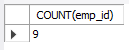
\includegraphics[width=0.4\textwidth]{./Figs/2020-12-24-20-58-35.png}
        % 	\caption{}
        \end{figure}
    
    \item Find how many employees have supervisors:
        \begin{minted}[autogobble]{sql}
            SELECT COUNT(super_id) FROM employee;
        \end{minted}
        \begin{figure}[H]
            \centering
            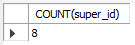
\includegraphics[width=0.4\textwidth]{./Figs/2020-12-24-20-53-55.png}
        % 	\caption{}
        \end{figure}
    
    \item Find the number of female employees born after 1970:
        \begin{minted}[autogobble]{sql}
            SELECT COUNT(emp_id) FROM employee WHERE sex = 'F' AND birth_day > '1971-01-01';
        \end{minted}
        \begin{figure}[H]
            \centering
            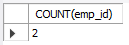
\includegraphics[width=0.4\textwidth]{./Figs/2020-12-24-20-57-32.png}
        % 	\caption{}
        \end{figure}
    
    \item Find the average of all employee's salaries:
        \begin{minted}[autogobble]{sql}
            SELECT AVG(salary) FROM employee;
        \end{minted}
        \begin{figure}[H]
            \centering
            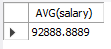
\includegraphics[width=0.4\textwidth]{./Figs/2020-12-24-20-54-52.png}
        % 	\caption{}
        \end{figure}
    
    \item Find the average of all employee's salaries who are male:
        \begin{minted}[autogobble]{sql}
            SELECT AVG(salary) FROM employee WHERE sex = 'M';
        \end{minted}
        \begin{figure}[H]
            \centering
            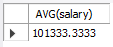
\includegraphics[width=0.4\textwidth]{./Figs/2020-12-24-20-55-56.png}
        % 	\caption{}
        \end{figure}
    
    \item Find the sum of all employee's salaries:
        \begin{minted}[autogobble]{sql}
            SELECT SUM(salary) FROM employee;
        \end{minted}
        \begin{figure}[H]
            \centering
            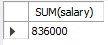
\includegraphics[width=0.4\textwidth]{./Figs/2020-12-24-20-55-34.png}
        % 	\caption{}
        \end{figure}
    
    \item Find out how many males and how many females there are:
        \begin{minted}[autogobble]{sql}
            SELECT COUNT(sex), sex FROM employee GROUP BY sex;
        \end{minted}
        \begin{figure}[H]
            \centering
            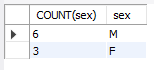
\includegraphics[width=0.4\textwidth]{./Figs/2020-12-24-20-58-58.png}
        % 	\caption{}
        \end{figure}
        \begin{itemize}
            \item This is called aggregation.
            \item The \mintinline{sql}{GROUP BY} allows us to display the count(sex) and sex in columns so that we can see what number belongs to what.
        \end{itemize}
    
    \item Find the total sales of each salesman:
        \begin{minted}[autogobble]{sql}
            SELECT SUM(total_sales), emp_id FROM works_with GROUP BY emp_id;
        \end{minted}
        \begin{figure}[H]
            \centering
            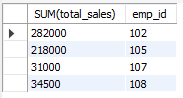
\includegraphics[width=0.4\textwidth]{./Figs/2020-12-24-20-59-32.png}
        % 	\caption{}
        \end{figure}
    
    \item Find the total purchases made from clients:
        \begin{minted}[autogobble]{sql}
            SELECT SUM(total_sales), emp_id FROM works_with GROUP BY client_id;
        \end{minted}
        \begin{figure}[H]
            \centering
            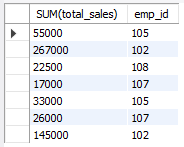
\includegraphics[width=0.4\textwidth]{./Figs/2020-12-24-20-59-59.png}
        % 	\caption{}
        \end{figure}
\end{itemize}
